% hyperref is loaded by the sn-jnl class; pass options before \documentclass to avoid option clashes
\PassOptionsToPackage{bookmarksdepth=4}{hyperref}
\documentclass[pdflatex]{sn-jnl}
\usepackage{float}

\usepackage[utf8]{inputenc}
\usepackage[T1]{fontenc}
\usepackage{lmodern}
\usepackage{microtype}

% DMKD figure-caption requirement: bold "Fig." and bold number, no colon
\usepackage[labelsep=space]{caption}
\captionsetup{compatibility=false}
\DeclareCaptionLabelFormat{dmkdfig}{\textsf{\textbf{#1~#2}}}
\AtBeginDocument{\captionsetup[figure]{name=Fig.,labelformat=dmkdfig}}

\usepackage{amsmath,amssymb}
\usepackage{booktabs}
% sn-jnl controls the page layout; avoid overriding margins via geometry.
% \usepackage{geometry}
\usepackage{array}
\usepackage{tabularx}
\usepackage{natbib} % ensure natbib is loaded for \setcitestyle
\setcitestyle{aysep={ }} % author-year citations without a comma (e.g., \citep{tashman2000} -> (Tashman 2000)
\Urlmuskip=0mu plus 1mu
\usepackage{graphicx}
\graphicspath{{figures/}}

% Reduce (or silence) underfull/overfull line warnings without changing wording
\pretolerance=1000
\tolerance=2000
\setlength{\emergencystretch}{3em}
\hbadness=10000

\title[Baseline-relative predictability horizons]{Baseline-Relative Predictability Horizons for Cross-Domain Forecast Evaluation}
\author*[1]{Federico Garcia Crespi}
\affil[1]{Departamento de Ingenier\'ia de Computadores, Universidad Miguel Hern\'andez, Elche, Spain}
\email{fedeg@umh.es}

\abstract{Forecasting studies are typically summarized at a few fixed lead times,
which can obscure the practical question of how long a method remains useful
relative to an explicit baseline. We recast predictability-horizon
estimation as a forecast evaluation task and measure baseline-relative
performance through the forecast skill curve $\mathrm{Skill}(h)$, obtained
using a leakage-free rolling-origin procedure with persistence as the
reference. To distinguish sporadic from sustained benefits, we report two
complementary horizon descriptors: $H^*(\mathrm{relax})$, the maximum
evaluated horizon such that $\mathrm{Skill}(h)>0$ (allowing intermediate
non-positive gaps), and $H^*(\mathrm{strict})$, the length of the longest
contiguous interval of positive skill. When needed (especially for
fragmented or late-recovery profiles), we additionally report interval
locations and sign-change structures. A pre-specified seasonal-persistence
sensitivity is evaluated on exact common support. It changes strict continuity
and interval location in several domains even when relaxed reach is unchanged,
confirming that the descriptors are baseline-conditional. Across the four settings, the empirical
results reveal distinct horizon-wise skill-profile patterns: immediate skill
collapse in electric load, delayed onset in PM$_{2.5}$, sustained positive skill
in wind speed, and fragmented positive intervals in traffic speed. These
contrasting patterns motivate reporting multiple operational
descriptors beyond fixed-horizon error summaries so that total positive reach,
sustained contiguous usefulness, and fragmented interval structure can be
distinguished under a shared leakage-free protocol.}

\keywords{forecast evaluation; predictability horizon; baseline-relative skill; rolling-origin evaluation; cross-domain forecasting}

\begin{document}
\maketitle




\section{Introduction}

In applied forecasting, evaluation is often reported at a small number of fixed lead times. This practice can obscure when (and for how long) a method is operationally useful relative to a strong baseline, especially when multi-step performance is non-monotonic or fragmented across the horizon. Methodological audits also document recurrent evaluation failures—including temporally invalid partitioning, leakage-prone preprocessing, omitted parsimonious baselines, and uncritical metric selection—that can materially distort conclusions about practical forecasting value \citep{hewamalage2023dmkd}. Yet cross-domain studies that quantify baseline-relative usefulness over the full forecast horizon under a shared, leakage-free protocol remain comparatively uncommon.

We address this gap with leakage-free rolling-origin evaluation, train-only preprocessing, and persistence as an explicit reference baseline. Horizon-wise baseline-relative performance is reported as skill curves $\mathrm{Skill}(h)$, and operational reach is summarized using complementary horizon descriptors that separate total positive reach from sustained contiguous usefulness.

We frame predictability-horizon estimation as an evaluation-methodology contribution for forecasting systems in machine learning and data mining. The goal is not to create another applied leader board, but to establish a protocol for characterizing and comparing useful predictive reach by horizon relative to a clearly specified baseline, thereby complementing recent methodological work on multi-step forecasting \citep{green2025stratify,kreuzer2025trend}.

Empirically, we apply this unified evaluation design to four domains—PM$_{2.5}$ air quality, electric load, wind speed, and traffic speed—chosen to span heterogeneous dynamics and baseline competitiveness under the same leakage-free protocol.

The paper makes three contributions:
\begin{enumerate}
  \item \textbf{A reproducible leakage-free evaluation framework:} we specify a rolling-origin protocol with train-only preprocessing that computes horizon-wise skill $\mathrm{Skill}(h)$ relative to an explicit persistence baseline, enabling comparable operational assessments across domains.
  \item \textbf{Operational horizon descriptors for useful predictive reach and continuity:} we instantiate the generic predictability-horizon concept via two complementary descriptors—$H^*(\mathrm{relax})$, the maximum evaluated horizon such that $\mathrm{Skill}(h)>0$ (allowing intermediate non-positive gaps), and $H^*(\mathrm{strict})$, the length of the longest contiguous positive-skill interval $[h_{\mathrm{start}},h_{\mathrm{end}}]$—augmented, when needed, with interval locations and sign-change structure for fragmented or late-recovery profiles.
  \item \textbf{A cross-domain empirical analysis under a shared protocol:} we show that domains differ not only in positive reach but also in continuity and fragmentation, and we quantify how the descriptors change under a pre-specified alternative baseline on exact common support.
\end{enumerate}

Together, these contributions provide a leakage-free, baseline-relative basis for estimating and comparing operational predictability horizons across domains.


\section{Related Work}

\subsection{Forecast evaluation metrics}

Within the forecasting literature, forecast evaluation is most often framed in terms of
accuracy metrics such as MAE and RMSE, along with scaled or relative variants that enable
comparisons across different series and applications. \citet{hyndman2006} survey
the most commonly used measures and underscore that no single metric is universally ideal;
the appropriate choice depends on scale, loss asymmetry, and the decisions the forecasts are
intended to inform \citep{petropoulos2022}.

For probabilistic forecasts, evaluation is commonly grounded in strictly proper scoring rules,
which ensure that the expected score is optimized by the forecaster's true predictive
distribution \citep{gneiting2007}. This framework shifts the evaluation focus from
point accuracy to the full predictive distribution, but the predominant empirical convention
remains point-forecast-based reporting at fixed horizons.

When comparing forecasting methods, statistical tests of predictive accuracy (e.g., the
Diebold--Mariano framework) are also frequently used to assess whether observed differences
are larger than would be expected by chance \citep{diebold1995}. This work does not
employ formal significance tests; instead, skill is assessed relative to explicit
baselines across the full set of evaluated horizons, with baseline sensitivity
evaluated on exact common support.

Empirical work typically reports errors for one or a few fixed horizons. While convenient, this fixed-horizon focus can hide how performance changes with lead time, including non-monotonic, fragmented, or delayed skill profiles in multi-step settings. Operationally, it can therefore be unclear whether a method is unhelpful overall or whether it provides baseline-relative usefulness only over specific horizon intervals. Fixed-horizon reporting also makes it difficult to directly identify where horizon-wise skill becomes non-positive relative to an explicit baseline.

Large-scale benchmark exercises have reinforced this convention.
Comparisons such as the M4 competition \citep{makridakis2020} and
repositories like the Monash Time Series Forecasting Archive
\citep{godahewa2021} assess many methods over many series, but usually
at fixed or pre-chosen horizons. This setup is effective for contrasting
methods on relative accuracy; yet, it does not directly characterize
how forecast skill evolves over the full horizon range or at which point
baseline-relative skill is exhausted.

A further drawback of fixed-horizon summaries is that, even when a
strong baseline is available, they only indirectly address operational
relevance. From an applied standpoint, the key question is often not
whether a method lowers error at a single, predefined horizon, but
whether it consistently improves on a baseline across the set of
horizons that matter for planning, control, or service-level agreements.
\citet{hyndman2018} consolidates prevailing guidance on forecast
evaluation and highlights the need for out-of-sample validation and for
matching the evaluation design to how forecasts are generated and used.
This points to evaluation constructs that summarize performance over
horizons and that are interpretable relative to a clearly specified
reference forecast.
Related methodological audits emphasize that common evaluation pitfalls (e.g., leakage-prone splits and missing strong baselines) can materially distort conclusions about practical forecasting value \citep{hewamalage2023dmkd}; we use this as motivation for the leakage-free, baseline-relative protocol described in Section~4.

\subsection{Forecast skill evaluation}

Baseline-relative evaluation is often expressed in terms of forecast
skill, which measures the error of a candidate forecasting method
against that of a reference forecast:
\begin{equation}
\mathrm{Skill}(h) = 1 - \frac{E_{\mathrm{model}}(h)}{E_{\mathrm{baseline}}(h)}.
\end{equation}
This representation is fundamental in forecast verification, where the
quality of a forecast is defined only in relation to a baseline
\citep{murphy1993}. In practical forecasting settings, the same rationale
underpins operational interpretation: a model that marginally improves
absolute error may still be operationally unimportant if it does not
surpass a strong baseline at the horizons that matter, whereas a model
whose gains appear only after a period of short-horizon baseline
dominance can still be highly useful for longer-range decision-making.

Skill-based reporting aligns naturally with multi-horizon evaluation
because it produces a horizon-specific quantity, the skill curve
$\mathrm{Skill}(h)$, instead of a single aggregate metric. This
facilitates distinguishing between evaluation outcomes driven by the
strength of the baseline and those stemming from modeling decisions. It
also underscores the importance of rigorous temporal evaluation
protocols. Out-of-sample forecast tests are typically implemented via
time-aware designs such as rolling-origin evaluation, which repeatedly
re-fits models and scores forecasts as the forecast origin moves forward
in time \citep{tashman2000}. These designs mirror real forecasting
practice and mitigate the risk that conclusions hinge on a particular
train--test split. The suitability of rolling-origin designs, in
contrast to blocked or random cross-validation for time series, has been
investigated empirically, with evidence indicating that respecting
temporal order is crucial for reliable performance estimation
\citep{cerqueira2020, bergmeir2012}.

In machine-learning-based forecasting, this principle is coupled with a
further practical issue: preventing temporal leakage arising from
preprocessing, feature engineering, hyperparameter tuning, or validation
procedures that inadvertently exploit future information~\citep{kapoor2023leakage}. Such leakage
can artificially boost apparent skill, especially at short horizons where
persistence effects are strong and where small misalignments or
preprocessing-related leakage can dominate evaluation results. Therefore,
leakage-free temporal validation is essential for interpreting skill
curves and for using baseline-relative evaluation to draw operational
conclusions about when forecasts are genuinely beneficial.

\subsection{Predictability limits}

Finite predictability in complex systems has long been recognized as a
core issue in forecasting and dynamical systems. \citet{lorenz1969}
demonstrated that sensitivity to initial conditions can create inherent
constraints on the lead times over which accurate prediction is
achievable. In empirical forecasting, similar limitations appear as the
horizon grows and the baseline becomes increasingly difficult to surpass.
However, these limits are not solely characteristics of a particular
model class; they emerge from the interplay among the system's dynamics,
the choice of reference forecast, and the evaluation protocol.

Fixed-horizon accuracy metrics remain the dominant reporting convention~\citep{makridakis2020,godahewa2021},
but they do not directly identify the horizon at which baseline-relative
skill is exhausted. From an operational standpoint, the key quantity is
the range of horizons over which a method achieves positive skill
relative to a baseline, under a clearly specified, temporally coherent
evaluation design.

A further limitation is comparability across heterogeneous domains.
Although baseline-relative skill measures are well established
\citep{hyndman2006, murphy1993, tashman2000}, the literature less
frequently provides cross-domain descriptions of practically useful
predictability horizons under a shared, leakage-free protocol. Large
benchmark studies \citep{makridakis2020, godahewa2021} compare methods
based on accuracy, but typically do not interpret the results as
operational estimates of when baseline-relative skill is depleted.

Without such a shared protocol, it remains unclear whether differences in
reported predictability across domains reflect genuine differences in system
dynamics and baseline competitiveness, or merely reflect inconsistencies in
evaluation design, preprocessing choices, or baseline specification.
This gap motivates baseline-relative horizon descriptors that summarize
the span of positive skill in a way that is robust to fragmented or
slowly emerging skill profiles and that supports comparison across
forecasting systems without conflating predictability with
methodological novelty or dataset-specific tuning.

\section{Problem Formulation}

Consider a time series $y_t$, $t = 1,\dots,T$.
A forecasting model generates predictions
\begin{equation}
\hat{y}_{t+h} = f_{\theta}(y_t, \dots, y_{t-L+1}),
\end{equation}
where $L$ denotes the input window length and $h$ the forecast horizon.
The corresponding forecast error is
\begin{equation}
e_{t,h} = y_{t+h} - \hat{y}_{t+h}.
\end{equation}
An aggregated error measure at horizon $h$ is given by $E(h)$, for
example, MAE or RMSE. A baseline forecasting method $b(\cdot)$ induces
a baseline error curve $E_{\mathrm{baseline}}(h)$.

\subsection{Operational Predictability Horizon}
In this work, operational predictability is understood as the range of time over which a forecasting system maintains positive skill relative to an explicit baseline, under a fixed, leakage-free evaluation setup.

We use $H^*$ as the generic conceptual notation for the operational predictability horizon: the maximum forecast horizon at which a model maintains positive skill relative to an explicit baseline under a specified evaluation protocol. Formally, the generic \emph{Forecast Skill Horizon} is
\begin{equation}
  H^* = \max \left\{ h \in \mathcal{H} : \mathrm{Skill}(h) > 0 \right\},
  \qquad
  \mathrm{Skill}(h) = 1 - \frac{E_{\mathrm{model}}(h)}{E_{\mathrm{baseline}}(h)}.
\end{equation}
Here, $\mathcal{H}$ denotes the set of evaluated forecast horizons. $H^*$ is protocol-defined: its value depends on the baseline choice (persistence in the primary analysis), preprocessing strategy, error metric, evaluated support, and evaluation scheme (leakage-free rolling-origin). This dependency is intentional, as it makes the descriptor reproducible and operationally interpretable.

\paragraph{Operational definitions:}
In empirical multi-step settings, $\mathrm{Skill}(h)$ curves may be
non-monotonic, fragmented, or exhibit delayed recovery, so the single
generic definition above is best treated as a conceptual anchor.
For example, a curve with early negative skill but a late positive
recovery yields a large $H^*(\mathrm{relax})$ but a short
$H^*(\mathrm{strict})$—two descriptors that a single maximum-horizon
summary conflates.

We therefore instantiate $H^*$ through two complementary reported
descriptors, defined over the evaluated horizon set
$\mathcal{H} = \{1, 2, \dots, H_{\max}\}$ and the positive-skill
subset $\mathcal{H}^+ = \{h \in \mathcal{H} \mid \mathrm{Skill}(h) > 0\}$. In the remainder of the paper, $H^*$ is used as the generic conceptual label for the operational predictability horizon, whereas all empirical reporting is based on the two instantiated descriptors $H^*(\mathrm{relax})$ and $H^*(\mathrm{strict})$.



\textbf{$H^*(\mathrm{relax})$:} The relaxed horizon is the maximum
evaluated horizon such that $\mathrm{Skill}(h)>0$, allowing intermediate
horizons with non-positive skill.
\begin{equation}
  H^*(\mathrm{relax}) = \max\!\bigl(\mathcal{H}^+ \cup \{0\}\bigr).
\end{equation}
Intermediate horizons with $\mathrm{Skill}(h)\leq 0$ may therefore lie
inside the relaxed reach, but those intermediate horizons are not
themselves interpreted as skillful horizons.

\textbf{$H^*(\mathrm{strict})$:} To capture sustained usefulness, let
$\mathcal{I}$ be the collection of all contiguous integer intervals
$I=[h_{\mathrm{start}},h_{\mathrm{end}}]$ with $I\subseteq\mathcal{H}^+$.
The strict horizon is the \emph{length} of the longest such interval:
\begin{equation}
  H^*(\mathrm{strict}) = \max_{I\in\mathcal{I}} |I|,
  \qquad |I| = h_{\mathrm{end}} - h_{\mathrm{start}} + 1.
\end{equation}
We additionally report the maximizing interval location
$[h_{\mathrm{start}}, h_{\mathrm{end}}]$ and, for fragmented or
late-recovery profiles, the full sign-change structure of
$\mathrm{Skill}(h)$. If several intervals tie for maximum length, the
earliest interval is reported. $H^*(\mathrm{time})$ denotes the wall-clock
duration corresponding to $H^*(\mathrm{strict})$ (not to
$H^*(\mathrm{relax})$), and it is reported alongside it.

Together, these two descriptors distinguish total positive reach from
sustained contiguous usefulness — a distinction that matters in the
fragmented and delayed-onset domains studied below.
Figure~\ref{fig:hstar_conceptual} illustrates this distinction: relaxed
reach extends to the last positive-skill horizon even when intervening
gaps occur, whereas strict reach measures the longest uninterrupted
positive-skill interval.

\begin{figure}[t]
  \centering
  
\includegraphics[width=0.82\textwidth]{fig_hstar_conceptual}
  \caption{Conceptual illustration of a baseline-relative skill curve $\mathrm{Skill}(h)$ with both positive and negative regions. The relaxed horizon $H^*(\mathrm{relax})$ is the maximum evaluated horizon with $\mathrm{Skill}(h) > 0$, whereas the strict horizon $H^*(\mathrm{strict})$ is the length of the longest contiguous positive-skill interval $[h_{\mathrm{start}},h_{\mathrm{end}}]$.}
  \label{fig:hstar_conceptual}
\end{figure}

\subsection{Operational interpretation and actionability}
$H^*(\mathrm{relax})$ describes the outer extent at which positive
baseline-relative skill is still observed; it does not license forecasts
at every preceding horizon. $H^*(\mathrm{strict})$, reported together
with $[h_{\mathrm{start}},h_{\mathrm{end}}]$, identifies the longest
continuous decision-relevant window in which the model improves on the
chosen baseline. Fixed-horizon summaries cannot reveal delayed onset,
intermediate gaps, fragmented positive islands, interval location, or
late recovery. The two descriptors therefore answer different operational
questions: how far any positive skill reaches, and where the longest
continuous useful window lies.

\section{Evaluation Framework}
This section specifies the evaluation components used to compute horizon-wise baseline-relative skill curves $\mathrm{Skill}(h)$ and the associated horizon descriptors: the reference baseline, error metrics, and the leakage-free rolling-origin validation protocol.

\subsection{Baseline models}

In every domain, we evaluate models against a persistence baseline. At forecast origin $t$, the baseline prediction for horizon $h$ is simply the most recent observation available at time $t$. Persistence is intentionally adopted as a strong operational reference because it is easy to implement, transparent, and often highly competitive for short lead times~\citep{murphy1993,hyndman2018}. Accordingly, the evaluation objective is not just to report absolute error levels but to determine the horizons at which a forecasting method yields positive skill relative to this baseline.

To assess baseline sensitivity, we additionally pre-specify seasonal
persistence before examining its results:
\begin{equation}
  \hat y^{\mathrm{season}}_{t+h}=y_{t+h-k_hs},
  \qquad k_h=\left\lceil\frac{h}{s}\right\rceil,
\end{equation}
where $s=24$ observations in the three hourly domains and $s=7$ in daily
electric load. The ceiling term selects the latest observation at the same
seasonal phase as the target that is available no later than origin $t$,
including when $h>s$. The period is fixed from sampling frequency and calendar
structure, not selected from evaluation performance. For this sensitivity,
LightGBM, persistence, and seasonal persistence are regenerated together, and
comparisons are permitted only when forecast origin, target timestamp, horizon,
and $y_{\mathrm{true}}$ match exactly. We report the number of records retained
on this common support.
At horizons that are exact multiples of $s$, this seasonal rule reduces to
$y_t$ and therefore coincides with ordinary persistence. Consequently, an
unchanged relaxed endpoint at such a horizon is partly structural and is not
interpreted as baseline invariance; changes in continuity and interval location
remain informative.

\subsection{Evaluation metrics}

Forecast errors are evaluated primarily using mean absolute error (MAE) \citep{hyndman2006}, which serves as the basis for computing baseline-relative skill at each horizon. Root mean squared error (RMSE) is additionally reported as a complementary error measure, but the main operational analysis throughout this work is framed in terms of $\mathrm{Skill}(h)$ computed from MAE. This design choice ensures that horizon-specific comparisons remain straightforward to interpret: at each lead time, we can directly assess whether a given forecasting approach improves upon persistence.

\subsection{Temporal validation protocol}
All experiments adopt rolling-origin evaluation with train-only preprocessing and persistence as the explicit reference baseline. This design yields leakage-free, out-of-sample horizon-wise skill estimates that are directly interpretable relative to a transparent, parsimonious operational baseline.
Figure~\ref{fig:rolling_origin} shows how the training information set,
forecast origin, and target horizons advance without exposing future
observations to model fitting or preprocessing.

\begin{figure}[t]
  \centering
  
\includegraphics[width=0.95\textwidth]{fig_rolling_origin_protocol}
  \caption{Schematic of the leakage-free rolling-origin evaluation protocol. Each origin uses a past-only training window with train-only preprocessing, generates $h$-step-ahead forecasts for the model and the persistence baseline, and then rolls the origin forward in time.}
  \label{fig:rolling_origin}
\end{figure}

All experiments use strictly time-ordered, leakage-free evaluation. The procedure adopts a rolling-origin framework~\citep{tashman2000}:
\begin{enumerate}
  \item define a chronologically ordered training window,
  \item fit any preprocessing steps using training data only,
  \item produce model and persistence forecasts for horizon $h$,
  \item advance the forecasting origin,
  \item iterate over all horizons and origins.
\end{enumerate}
Random train-test splits are intentionally avoided because they may introduce temporal leakage.
For all domains, model and baseline forecasts are generated and compared only at aligned timestamps.

\section{Datasets}

Table~\ref{tab:datasets} provides an overview of the application
domains, datasets, target variables, temporal resolution, and maximum
forecast horizon.

The four domains are selected to support methodological comparison under a
shared, leakage-free evaluation design rather than to provide exhaustive
coverage of forecasting applications. They span heterogeneous temporal
structures (from highly regular aggregate demand to intermittent traffic
and wind dynamics), differ markedly in baseline competitiveness against
persistence, and vary in temporal resolution and operational context
(hourly environmental and mobility signals versus a daily energy series).
Together, they form a diverse but controlled public cross-domain testbed
for studying horizon-wise baseline-relative skill and its summaries.

Under this shared protocol, the four domains yield distinct baseline-relative skill-curve profiles, enabling the comparison of operational reach, contiguous usefulness, and (when present) fragmented interval structure.

\begin{table}[h]
\centering
\small
\setlength{\tabcolsep}{3pt}
\begin{tabular}{lllll}
\toprule
Domain & Dataset & Variable & Frequency & $H_{\max}$ \\
\midrule
Air quality & UCI Beijing PM2.5 (2010--2014) & PM$_{2.5}$ & hourly & 48 \\
Energy & UCI Electricity Load Diagrams 2011--2014 & Aggregate load & daily & 1 \\
Wind & NREL Wind Toolkit & Wind speed & hourly & 48 \\
Traffic & PeMS / METR-LA & Traffic speed & hourly & 72 \\
\bottomrule
\end{tabular}
\caption{Public datasets used for cross-domain predictability analysis.
In the energy domain, we use the UCI Electricity Load Diagrams
2011--2014 dataset \citep{trindade2015}.
The aggregate daily series is obtained by summing all 370 client series
and resampling to daily totals, starting from 2013-03-06, which is the
first date with $\geq$90\% active clients over seven consecutive days.}
\label{tab:datasets}
\end{table}

In the traffic domain, the raw source variable corresponds to METR-LA
sensor speed measurements \citep{li2018dcrnn}.

\subsection{Data representation}

For each domain, the cleaned data used in the experiments is
standardized into a univariate format containing a timestamp column and
a single target variable. In the electric-load domain, the cleaned
representation is $(\texttt{timestamp}, \texttt{value})$ at daily
resolution. The aggregate series is defined as the daily sum of all
available client-level series from the stable-coverage start date
onward. This explicit specification of the aggregation procedure
promotes reproducibility and ensures alignment between data preparation
and experimental evaluation.

\section{Experimental Setup}

\subsection{Forecast horizons}

The maximum forecast horizons are chosen to balance practical
operational relevance with a sufficient length to capture the onset and
progression of skill decay:
\begin{itemize}
  \item PM$_{2.5}$: $H_{\max}=48$,
  \item Electric load (daily): $H_{\max}=1$,
  \item Wind: $H_{\max}=48$,
  \item Traffic: $H_{\max}=72$ (hourly).
\end{itemize}
When supported by operational considerations, these upper limits may
differ across domains. Nonetheless, the primary cross-domain analysis
is carried out over a shared interval, $h=1,\ldots,48$, to maintain
comparability among systems.

\subsection{Models}

The empirical study compares forecasting performance against an
explicit persistence baseline and employs LightGBM as the principal
forecasting model. Evaluation semantics are shared across domains, while
the fixed feature and estimator configurations follow the experiment
scripts that produced the submitted results.

LightGBM is a decision tree-based gradient boosting framework that is
particularly well suited for tabular, lag-based forecasting
formulations~\citep{ke2017lightgbm}. For the three hourly domains
(PM$_{2.5}$, wind, and traffic), the fixed configuration is:
\begin{itemize}
  \item input lags: $\{0,1,2,3,6,12,24,48\}$ relative to the forecasting origin,
  \item rolling-origin stride: 24,
  \item number of estimators: 50,
  \item learning rate: 0.05; number of leaves: 31; subsample and feature
  fractions: 0.9; random seed: 42.
\end{itemize}
Lag 0 ($y_t$) is included so that the model and baseline share the same
information at the forecasting origin; this does not introduce leakage
since the target remains $y_{t+h}$ for $h \geq 1$.
The daily electric-load experiment uses the fixed historical producer
configuration: 14 daily lags plus day of week, a 365-day rolling training
window, 100 estimators, learning rate 0.05, 15 leaves, and random seed 42.
These configurations were not selected by tuning on the evaluation period.

The persistence baseline is defined as the most recent observed value
available at the prediction origin.
\begin{equation}
\hat{y}^{\mathrm{base}}_{t+h} = y_t,
\end{equation}
and is applied uniformly in all domains. This baseline is deliberately
strong in operational forecasting contexts and serves as the reference
level against which baseline-relative usefulness is assessed.
Table~\ref{tab:baseline_domains} summarizes the baseline definition and an
illustrative domain-specific example. Units follow the corresponding source
metadata; for electric load, the historical producer sums 15-minute kW
readings, so division by four expresses the stored aggregate as kWh.

\begin{table*}[htbp]
\centering
\footnotesize
\setlength{\tabcolsep}{4pt}
\renewcommand{\arraystretch}{1.18}
\begin{tabularx}{\textwidth}{@{}p{1.45cm} p{2.55cm} p{3.2cm} X@{}}
\toprule
\textbf{Domain} & \textbf{Target unit} & \textbf{Persistence rule} & \textbf{Illustrative explanation} \\
\midrule
PM$_{2.5}$ & $\mu\mathrm{g}\,\mathrm{m}^{-3}$ & $\hat y_{t+h}^{\mathrm{base}}=y_t$ & If $y_t=42\,\mu\mathrm{g}\,\mathrm{m}^{-3}$, every lead uses $42\,\mu\mathrm{g}\,\mathrm{m}^{-3}$. \\
Load & Sum of 15-min kW readings & $\hat y_{t+h}^{\mathrm{base}}=y_t$ & The stored daily aggregate follows the producer script; dividing it by four gives the equivalent energy in kWh. \\
Wind & $\mathrm{m}\,\mathrm{s}^{-1}$ at 100 m & $\hat y_{t+h}^{\mathrm{base}}=y_t$ & If $y_t=6.8\,\mathrm{m}\,\mathrm{s}^{-1}$, every lead uses $6.8\,\mathrm{m}\,\mathrm{s}^{-1}$. \\
Traffic & mph & $\hat y_{t+h}^{\mathrm{base}}=y_t$ & If $y_t=57$ mph, every lead uses 57 mph. \\
\bottomrule
\end{tabularx}
\caption{Persistence definition and verified target units in each domain. Electric-load values are retained on the exact scale produced by the historical aggregation script; the stated conversion follows the source dataset's 15-minute kW sampling.}
\label{tab:baseline_domains}
\end{table*}


No hyperparameter tuning is carried out in any domain. The protocol is
kept deliberately simple so that observed differences in skill reflect
domain characteristics and baseline competitiveness rather than model
optimization. The exact fixed configuration used in each domain is reported
above and retained for reproducibility; no claim of identical feature
construction across hourly and daily domains is made.

\subsection{Reproducibility rules}

All tables and figures are generated directly from the experiments
carried out under the stated evaluation protocol. To support
replication, the data-processing and evaluation scripts operate on the
cleaned, domain-specific datasets, with each step documented so that
the reported results can be reproduced from the specified inputs.


\section{PM$_{2.5}$ Domain Results}

\subsection{\texorpdfstring{PM$_{2.5}$}{PM2.5} experimental setting}

The first domain we analyze is the Beijing PM$_{2.5}$ forecasting case \citep{chen2015beijingpm25}, which provides an initial empirical demonstration of the proposed evaluation framework. The study relies on hourly measurements, a persistence baseline, and the standard comparable LightGBM setup with $H_{\max}=48$, using MAE-based skill for horizon-wise assessment. This domain is particularly informative for highlighting settings in which persistence remains very strong at short lead times, and positive skill appears only at longer horizons.

\subsection{Observed skill behavior}
For PM$_{2.5}$, the $\mathrm{Skill}(h)$ curve in
Figure~\ref{fig:skill-pm25} shows a delayed, contiguous interval of positive
skill following a long region of negative skill. Under the main protocol,
this yields $H^*(\mathrm{relax}) = 48$, $H^*(\mathrm{strict}) = 13$, and a
longest positive interval $[h_{\mathrm{start}},h_{\mathrm{end}}] = [36, 48]$,
with $H^*(\mathrm{time}) = 13$ h.

\subsection{Interpretation}
The relaxed descriptor reaches the maximum evaluated horizon because positive skill is observed at $h=48$, even though the early region is negative. The strict descriptor is shorter because it measures sustained usefulness and is determined by the longest contiguous positive-skill interval, here $[36,48]$ with a length of 13. Operationally, PM$_{2.5}$ represents delayed contiguous emergence: baseline-relative usefulness appears late and persists continuously once it appears. Additional second-model artifacts for PM$_{2.5}$ (XGBoost) are available, but they are treated as qualitative support unless strict protocol comparability is explicitly documented.
\begin{figure}[t]
  \centering
  
\includegraphics[width=0.88\textwidth]{fig_skill_pm25.pdf}
  \caption{PM$_{2.5}$ skill curve $\mathrm{Skill}(h)$ under the leakage-free rolling-origin protocol. The skill-profile pattern shows delayed onset: persistence dominates at short lead times and positive skill emerges only at longer horizons.}
  \label{fig:skill-pm25}
\end{figure}


\section{Electric Load Domain Results}

\subsection{Energy experimental setting}

The second domain considered is aggregate daily electricity demand, derived from the UCI Electricity Load Diagrams 2011--2014 dataset. This experiment uses daily observations, a persistence baseline, and the canonical comparable LightGBM protocol, with performance evaluated through MAE-based skill. The energy setting is especially informative because the series is highly regular, and persistence is expected to be particularly difficult to outperform; more broadly, electric load forecasting is a canonical operational setting where benchmarking and uncertainty-aware evaluation are central concerns \citep{hong2016}.

\subsection{Observed skill behavior}
In the canonical reported setting, daily electric load is operationally summarized at $h = 1$, yielding $H^*(\mathrm{relax}) = 1$ and $H^*(\mathrm{strict}) = 1$ with $[h_{\mathrm{start}},h_{\mathrm{end}}] = [1, 1]$. For visualization purposes, Figure~\ref{fig:skill_load} additionally shows an auxiliary extended-horizon view up to $h=7$ under the same protocol, highlighting that positive skill against persistence decays rapidly and remains confined to a very short early interval.
Both operational variants yield the same result:
\begin{equation}
H^*(\mathrm{relax}) = 1, \qquad H^*(\mathrm{strict}) = 1, \qquad [h_{\mathrm{start}}, h_{\mathrm{end}}] = [1,1], \qquad H^*(\mathrm{time}) = 1\ \mathrm{day}.
\end{equation}

\subsection{Interpretation}
The aggregate daily electricity demand series exhibits low relative variability (CV$\approx$0.16) and strong day-to-day autocorrelation (ACF lag-1$\approx$0.92), both of which make the last-observation-carried-forward persistence forecast particularly difficult to improve upon at the daily scale. With only $h=1$ evaluated, $H^*(\mathrm{relax})$ and $H^*(\mathrm{strict})$ coincide by construction and reflect that positive skill is observed on the first (and only) evaluated day. Operationally, this domain represents an immediate collapse under strong persistence dominance: any baseline-relative advantage is confined to the earliest evaluated step. Qualitatively similar conclusions are also supported by a simple moving-average comparison, but this is not treated as a strict protocol-matched robustness check.
\begin{figure}[t]
  \centering
  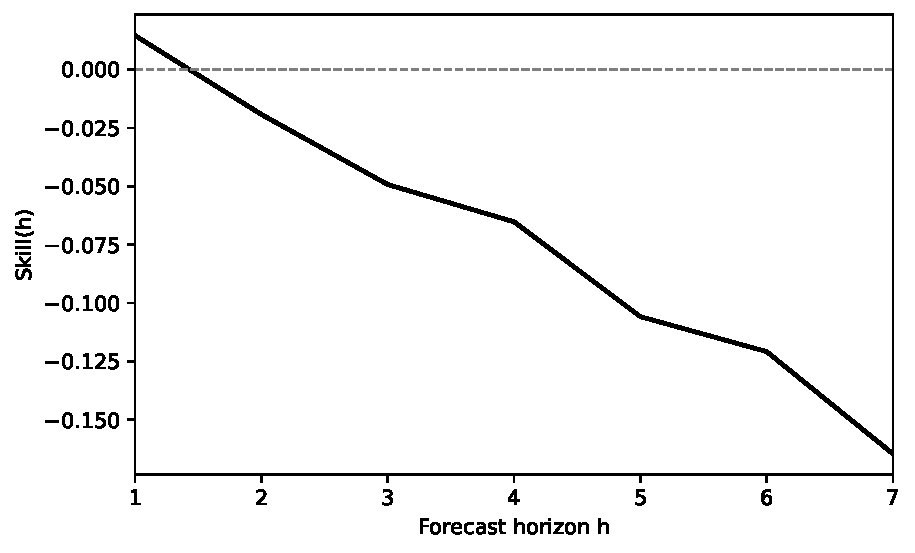
\includegraphics[width=0.88\textwidth]{fig_skill_load.pdf}
  \caption{Electric-load skill curve $\mathrm{Skill}(h)$ under the leakage-free rolling-origin protocol. The canonical cross-domain analysis uses $H_{\max}=1$, yielding $H^*(\mathrm{relax})=1$ and $H^*(\mathrm{strict})=1$ at $h=1$. The extended view up to $h=7$ is shown only to illustrate the rapid decay of positive skill against persistence beyond the first day.}
  \label{fig:skill_load}
\end{figure}


\section{Wind Domain Results}

\subsection{Wind experimental setting}

The third domain considered is the NREL Wind Toolkit \citep{draxl2015}, which provides hourly wind-speed time series. The wind experiment uses hourly observations, a persistence baseline, and the canonical comparable LightGBM protocol under $H_{\max}=48$, with performance again evaluated through MAE-based skill. This domain is included to assess whether the proposed horizon descriptors also characterize settings in which positive skill is sustained across most or all of the evaluated horizon range.

\subsection{Observed skill behavior}
For wind, positive skill is obtained over the entire set of evaluated horizons, yielding a uniformly positive skill curve across $h=1,\dots,48$ (Figure~\ref{fig:skill-wind}). This shape indicates comparatively weak baseline competitiveness: persistence is outperformed not only at longer lead times but also at the shortest horizons.
Under the operational variants examined in this study,
\begin{equation}
\begin{aligned}
H^*(\mathrm{relax}) &= 48, & [h_{\mathrm{start}}, h_{\mathrm{end}}] &= [1,48],\\
H^*(\mathrm{strict}) &= 48, & H^*(\mathrm{time}) &= 48\ \mathrm{h}.
\end{aligned}
\end{equation}

\subsection{Interpretation}
Because the skill curve remains positive throughout the evaluated range, $H^*(\mathrm{relax})$ and $H^*(\mathrm{strict})$ coincide and equal $H_{\max}$, and the maximizing interval is $[1,48]$. Operationally, wind represents sustained positive skill: the model retains baseline-relative usefulness continuously across the entire evaluated horizon range.

\begin{figure}[t]
  \centering
  
\includegraphics[width=0.88\textwidth]{fig_skill_wind.pdf}
  \caption{Wind skill curve $\mathrm{Skill}(h)$ under the leakage-free rolling-origin protocol. The skill-profile pattern shows sustained positive skill across the evaluated horizon range.}
  \label{fig:skill-wind}
\end{figure}

\section{Traffic Domain Results}

\subsection{Traffic experimental setting}

The fourth domain considered is the METR-LA hourly traffic-speed dataset \citep{li2018dcrnn}, constructed from a univariate sensor trajectory. The experiment uses hourly observations, a persistence baseline, and the canonical comparable LightGBM protocol, with MAE-based skill evaluated for forecasting horizons up to $H_{\max}=72$. This domain is especially suitable for studying fragmented skill profiles, in which predictive usefulness may arise in short, separated intervals rather than in a single sustained range.

\subsection{Observed skill behavior}
In the traffic domain, the skill curve is highly non-monotonic and fragmented under the canonical comparable LightGBM protocol (Figure~\ref{fig:skill-traffic}): positive skill appears in short, separated intervals interspersed with negative regions. This shape is consistent with strong baseline competitiveness at many horizons, punctuated by intermittent recoveries where the model surpasses persistence.
For LightGBM,
\begin{equation}
H^*(\mathrm{relax}) = 72, \qquad [h_{\mathrm{start}}, h_{\mathrm{end}}] = [46,52], \qquad H^*(\mathrm{strict}) = 7, \qquad H^*(\mathrm{time}) = 7\ \mathrm{h}.
\end{equation}
The first positive interval occurs at $[17,18]$, and the sign of $\mathrm{Skill}(h)$ changes 19 times across $h\in\{1,\dots,72\}$.

\subsection{Interpretation}
These results illustrate why multiple descriptors are needed in fragmented
settings. The relaxed descriptor records the last positive-skill horizon,
whereas the strict descriptor and its location reveal that the longest
continuous useful window is only seven hours and occurs at $[46,52]$.

\begin{figure}[t]
  \centering
  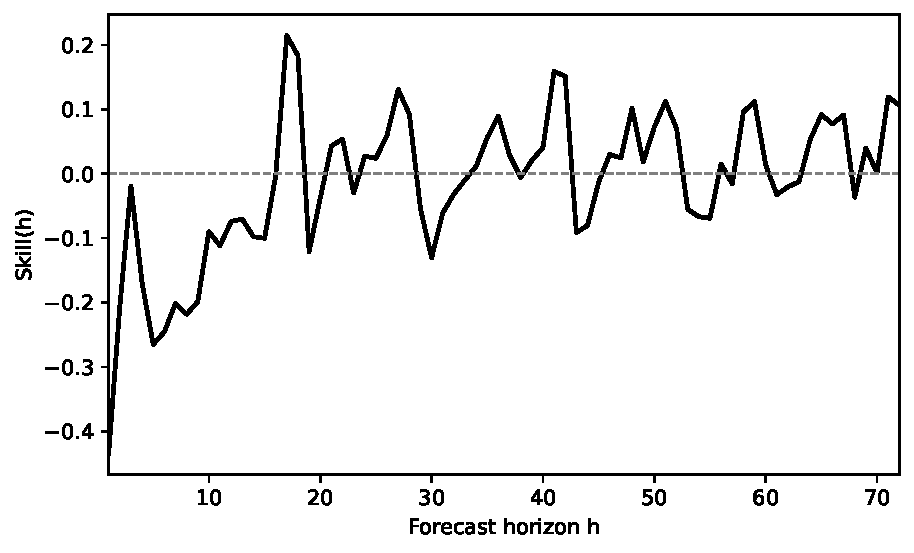
\includegraphics[width=0.88\textwidth]{fig_skill_traffic.pdf}
  \caption{Traffic skill curve $\mathrm{Skill}(h)$ under the leakage-free rolling-origin protocol. The skill-profile pattern shows fragmented positive intervals: brief, separated stretches of positive skill interspersed with negative regions.}
  \label{fig:skill-traffic}
\end{figure}

Table~\ref{tab:results} presents the operational horizon descriptors
derived for the four study domains under a common evaluation framework.
Together, these four domains instantiate qualitatively different horizon-wise skill structures under a shared, leakage-free evaluation design, which is why a single horizon summary is insufficient.
The comparison reveals four distinct patterns of predictability.
Electric load is characterized by immediate persistence dominance, with
positive skill confined to the first day. Traffic displays fragmented
predictability, where positive skill arises in short, isolated segments
rather than as a continuous region. PM$_{2.5}$ exhibits a delayed onset
of a contiguous interval of useful predictability, whereas wind
demonstrates the highest level of operational predictability,
maintaining positive skill across the entire evaluated horizon.
Collectively, these findings indicate that fixed-horizon summaries can
obscure substantial cross-domain variability in the structure of
baseline-relative predictability.

\begin{table}[h]
\centering
\small
\setlength{\tabcolsep}{4pt}
\renewcommand{\arraystretch}{1.1}
\begin{tabularx}{\linewidth}{@{}l c c >{\centering\arraybackslash}p{1.8cm} >{\centering\arraybackslash}p{1.4cm} >{\raggedright\arraybackslash}X@{}}
\toprule
Domain & $H^*(\mathrm{relax})$ & $H^*(\mathrm{strict})$ & $[h_{\mathrm{start}}, h_{\mathrm{end}}]$ & $H^*(\mathrm{time})$ & Notes \\
\midrule
PM$_{2.5}$ & 48 & 13 & $[36,48]$ & 13 h & strong persistence; contiguous positive-skill interval emerges late, following an extended negative region \\
Load (daily) & 1 & 1 & $[1,1]$ & 1 day & positive skill is confined to the first evaluated day under this setup \\
Wind & 48 & 48 & $[1,48]$ & 48 h & positive skill over the full evaluated range relative to persistence \\
Traffic & 72 & 7 & $[46,52]$ & 7 h & fragmented profile with 19 sign changes and first positive interval $[17,18]$ \\
\bottomrule
\end{tabularx}
\caption{Comparison of predictability horizons across domains (PM$_{2.5}$, electric load, wind, and traffic).}
\label{tab:results}
\end{table}

\subsection{Alternative-baseline sensitivity}
Table~\ref{tab:baseline-sensitivity} reports the pre-specified seasonal-
persistence sensitivity. Every row is computed from newly generated
per-origin forecasts after verifying exact equality of forecast origin, target
timestamp, horizon, and $y_{\mathrm{true}}$; no records are lost in the
pairwise alignments. Because PM$_{2.5}$ contains missing observations, its
persistence row on this common subset (48/22, $[27,48]$) differs from the
primary full-support persistence result (48/13, $[36,48]$). This is a support
effect and the sensitivity row does not replace the primary result.

Relative to the matched persistence row, seasonal persistence changes
$H^*(\mathrm{strict})$ from 22 to 24 in PM$_{2.5}$ and shifts the interval
from $[27,48]$ to $[25,48]$; load remains 1/1 at $[1,1]$; wind changes from
48 at $[1,48]$ to 30 at $[19,48]$; and traffic changes from 7 at $[46,52]$
to 14 at $[48,61]$. In all four domains $H^*(\mathrm{relax})$ is unchanged.
For the hourly domains, however, the evaluated endpoint is an exact multiple
of the 24-hour period, where seasonal persistence equals ordinary persistence;
the unchanged relaxed endpoint is therefore partly structural and is not
evidence of general baseline invariance. The changes in strict continuity and
interval location demonstrate the substantive baseline conditionality of the
descriptors.

\begin{table}[t]
\centering
\small
\setlength{\tabcolsep}{4pt}
\begin{tabular}{@{}llcccl@{}}
\toprule
Domain & Baseline & Common $n_h$ & $H^*_{\mathrm{relax}}$ & $H^*_{\mathrm{strict}}$ & Longest interval \\
\midrule
PM$_{2.5}$ & Persistence & 328--346 & 48 & 22 & $[27,48]$ \\
PM$_{2.5}$ & Seasonal persistence & 328--346 & 48 & 24 & $[25,48]$ \\
\addlinespace[2pt]
Load & Persistence & 301 & 1 & 1 & $[1,1]$ \\
Load & Seasonal persistence & 301 & 1 & 1 & $[1,1]$ \\
\addlinespace[2pt]
Wind & Persistence & 350--354 & 48 & 48 & $[1,48]$ \\
Wind & Seasonal persistence & 350--354 & 48 & 30 & $[19,48]$ \\
\addlinespace[2pt]
Traffic & Persistence & 102--108 & 72 & 7 & $[46,52]$ \\
Traffic & Seasonal persistence & 102--108 & 72 & 14 & $[48,61]$ \\
\bottomrule
\end{tabular}
\caption{Baseline sensitivity on exact common support. $n_h$ is the number of aligned forecast origins at each horizon (a range is shown when it varies with $h$). The persistence rows in this table are recomputed on the same support as seasonal persistence and therefore need not equal the primary full-support persistence descriptors.}
\label{tab:baseline-sensitivity}
\end{table}


\section{Discussion}
The four empirical results reveal qualitatively distinct horizon-wise skill-profile patterns that fixed-horizon accuracy summaries would not recover. In electric load, skill collapses immediately against persistence, leaving no operationally useful horizon beyond the first day. Traffic exhibits a fragmented structure: positive skill arises in short, isolated intervals separated by non-positive regions, so that $H^*(\mathrm{strict})$ is substantially shorter than $H^*(\mathrm{relax})$. PM$_{2.5}$ presents a delayed-emergence pattern in which persistence dominates at short lead times, but a contiguous interval of positive skill appears and stabilizes at longer horizons. Wind stands apart as the only domain with positive skill sustained across the entire evaluated range relative to persistence.

These empirical patterns can be read as four operational profile types under baseline-relative, horizon-wise evaluation: (i) immediate collapse under strong baseline competition (electric load), (ii) delayed but contiguous emergence of positive skill (PM$_{2.5}$), (iii) sustained positive skill across the evaluated horizon range (wind), and (iv) fragmented late recovery with model-sensitive continuity (traffic). The typology makes explicit why a single horizon summary is insufficient: $H^*(\mathrm{relax})$ alone can overstate operational usefulness in fragmented settings, while $H^*(\mathrm{strict})$ alone can miss delayed positive reach. Reporting both descriptors—and, when needed, interval locations and sign-change structure—provides a compact summary of reach and continuity.

These results also reinforce concerns raised in prior methodological work: fixed-horizon reporting can hide delayed or fragmented usefulness, and leakage-prone evaluation or missing strong baselines can distort conclusions about practical value. The persistence-relative rolling-origin design used here addresses both issues directly.

\textbf{Potential dynamic use.} An operational system could use an $H^*$
profile estimated on historical validation data to freeze a set of eligible
forecast horizons for subsequent deployment, and later update that policy
using only errors that have already been realised. This paper does not
validate such an adaptive controller. Re-estimating $H^*$, selecting horizons,
and evaluating that choice on the same errors would introduce adaptive
selection bias and overfitting. A dynamic policy therefore requires a
prospective, prequential, or nested evaluation in which horizon selection is
separated from the data used to assess it.

\textbf{Metric sensitivity.} The qualitative morphology of $\mathrm{Skill}(h)$ is not uniformly invariant to the choice of error metric: while PM$_{2.5}$ and wind retain their main profile types under RMSE, electric load and traffic change materially. This reinforces the interpretation of $H^*$ as a protocol-conditional descriptor rather than a quantity with universal cross-metric stability.

\textbf{Baseline sensitivity.} Seasonal persistence alters the longest
continuous positive-skill window in PM$_{2.5}$, wind, and traffic, despite
leaving relaxed reach unchanged in this design. Wind provides the clearest
example: the strict interval contracts from the full $[1,48]$ range under
persistence to $[19,48]$ under seasonal persistence. Traffic changes in the
opposite direction, from a seven-hour to a fourteen-hour longest interval.
These outcomes are reported without selecting the reference that gives a more
favourable profile and show why the baseline is part of the estimand.

\textbf{Scope of inference.} Because baseline competitiveness and evaluation design shape $\mathrm{Skill}(h)$, operational predictability horizons are not intrinsic properties of a forecasting model or domain. They reflect the interaction of dataset, model, baseline choice, metric, evaluated range, and temporal validation protocol.

These findings point to two methodological implications for horizon-based forecast evaluation:
\begin{enumerate}
  \item Predictability should be assessed relative to an explicit baseline; in cross-domain studies, using a common baseline is often essential for comparability.
  \item Horizon estimation should differentiate between relaxed and contiguous predictability, particularly when empirical skill curves are delayed or fragmented.
\end{enumerate}

Overall, fixed-horizon summaries lose structural information that matters operationally: fragmented or delayed profiles can yield the same fixed-horizon summary while implying very different decision windows. Reporting $H^*(\mathrm{relax})$ and $H^*(\mathrm{strict})$ together (and interval structure when needed) separates total positive reach from sustained usefulness while making explicit that any $H^*$ estimate is conditional on the baseline, metric, and evaluation protocol.

\section{Limitations}

The horizon descriptors reported in this paper should be interpreted as
\emph{operationally conditional} summaries rather than as universal
constants. Their values depend on the baseline choice, the maximum
evaluated horizon $H_{\max}$, dataset and domain properties, and the
evaluation design. Together, these factors determine what counts as
useful baseline-relative reach under a leakage-free protocol.
The empirical scope is limited to four datasets and their stated temporal
periods, the fixed LightGBM configurations reported above, and the evaluated
horizon caps. Results need not transfer to another dataset, target, model
configuration, baseline, metric, or $H_{\max}$. The alternative-baseline
sensitivity reported in the revision examines baseline conditionality but
does not eliminate it. Seasonal persistence also coincides with ordinary
persistence at exact multiples of the seasonal period, so unchanged terminal
reach at those endpoints is not an independent invariance result. Moreover, no dynamic $H^*$ controller is evaluated
prospectively; the operational policy described in the Discussion remains a
potential application requiring separate prequential or nested validation.

More formally, the horizon descriptors reported here should be understood as
\[
H^* = H^*(\text{dataset}, \text{model}, \text{baseline}, \text{metric}, \text{validation protocol}),
\]
rather than as intrinsic properties of a forecasting system. In particular, the metric-sensitivity analysis indicates that changing the error metric from MAE to RMSE can modify not only the numerical values of $H^*(\mathrm{relax})$ and $H^*(\mathrm{strict})$ but, in some domains, the qualitative morphology of $\mathrm{Skill}(h)$ itself. As a result, claims of cross-metric invariance are not warranted in general, and any reported horizon estimates should always be interpreted in the context of the full evaluation protocol.

These results show why $H^*(\mathrm{relax})$ alone is not sufficient in
fragmented settings. When skill curves are non-monotonic, total positive
reach can remain stable even though contiguous usefulness and interval
structure change across models. Reporting $H^*(\mathrm{strict})$,
together with interval locations and, when needed, sign-change
structure, therefore provides a more informative summary of operational
usefulness. Clear reporting of the baseline, evaluated horizon range,
dataset, model, and protocol remains necessary for reproducibility and
for the correct interpretation of any reported $H^*$ estimate.


\section{Conclusion}

This study frames predictability-horizon estimation as an operational
forecast-evaluation task, focused on skill relative to an explicit
baseline. The contribution is not a new forecasting model but a
leakage-free, baseline-relative way to summarize useful predictive reach
across horizons via the skill curve $\mathrm{Skill}(h)$.

Using rolling-origin evaluation against persistence, we report two
complementary horizon descriptors: $H^*(\mathrm{relax})$ (the maximum
evaluated horizon with any positive skill) and $H^*(\mathrm{strict})$
(the longest uninterrupted run of positive skill), augmented when needed
with interval locations and sign-change structure. Across the four
domains, useful predictive reach differs not only in extent but also in
continuity and fragmentation, and the baseline-sensitivity analysis makes
explicit that these descriptors are conditional on the chosen reference.
Future work will test whether these
operational skill-profile types recur systematically across broader
domain families and evaluation designs, and whether more expressive model
classes or multivariate formulations alter the interval structure of
baseline-relative usefulness.

\appendix

\subsection*{A.1 Metric sensitivity}

The main analysis in this paper is based on MAE-derived skill curves, which are a common choice for scale-dependent error evaluation in applied forecasting. To examine how the proposed horizon descriptors behave under a different loss geometry, we recomputed the skill curves using RMSE as the underlying error metric while keeping all other components of the protocol fixed (datasets, models, persistence baseline, and rolling-origin design).

The resulting metric sensitivity is heterogeneous across domains. In the electric-load domain, replacing MAE with RMSE extends the positive-skill region from the first horizon to a short early interval, yielding $H^*(\mathrm{relax})=3$, $H^*(\mathrm{strict})=3$, and $[h_{\mathrm{start}},h_{\mathrm{end}}]=[1,3]$ under the present configuration, without altering the broader impression that persistence dominates beyond very short lead times. In the traffic domain, the effect is considerably stronger: the MAE-based fragmented profile becomes a near-contiguous positive-skill regime under RMSE, with $H^*(\mathrm{relax})=72$, $H^*(\mathrm{strict})=63$, and the longest positive interval $[10,72]$, indicating that the qualitative morphology of $\mathrm{Skill}(h)$ itself can depend on the error metric.

By contrast, PM$_{2.5}$ and wind retain their main qualitative profile types under RMSE. For PM$_{2.5}$, RMSE preserves the delayed-emergence pattern, with $H^*(\mathrm{relax})=48$, $H^*(\mathrm{strict})=18$, and the longest positive interval $[31,48]$. For wind, the skill curve remains fully positive across the evaluated range, with $H^*(\mathrm{relax})=48$, $H^*(\mathrm{strict})=48$, and $[1,48]$. Taken together, these observations suggest that the proposed descriptors should be interpreted as protocol-conditional summaries: the choice of error metric is a substantive component of the operational definition of $H^*(\mathrm{relax})$ and $H^*(\mathrm{strict})$, rather than a secondary implementation detail, and cross-metric invariance cannot be assumed uniformly across domains.

\section*{Declarations}

\subsection*{Funding}
The author did not receive support from any organization for the submitted work.

\subsection*{Competing Interests}
The author has no competing interests to declare that are relevant to the content of this article.

\subsection*{Ethics Approval}
Not applicable. This study is based exclusively on publicly available benchmark datasets. It did not involve human participants, animals, patient data, or primary data collection.

\subsection*{Data Availability}
All datasets used in this study are publicly available. The replication package
accompanying this revision provides a single reproducibility entry point
(\texttt{data/README.md}) and a machine-
readable manifest (\texttt{data/MANIFEST.tsv}) record the source identifier,
expected SHA-256 checksum, preprocessing script, and redistribution status for
each of the four experimental inputs. The exact processed PM$_{2.5}$ and
electric-load inputs are versioned in the repository. Wind (NREL WTK-LED CONUS,
2019, point sample) and METR-LA are deterministically retrieved and processed by
the supplied retrieval script, which verifies their expected checksums; they are
not claimed to be repository-cached. The original sources remain the UCI
repositories for electric load~\citep{trindade2015} and Beijing
PM$_{2.5}$~\citep{chen2015beijingpm25}, NREL for wind~\citep{draxl2015}, and
the DCRNN/METR-LA distribution for traffic~\citep{li2018dcrnn}.

\subsection*{Code Availability}
The replication package accompanying this revision contains the data-processing,
forecasting, common-support validation, descriptor, table, and figure-generation
scripts used for the reported results. The public project location is
\url{https://github.com/EduIntellect/paper2H}.

\section*{Acknowledgments}
None.


% Springer/DMKD bibliography (BibTeX)
\bibliographystyle{sn-basic}
\bibliography{sn-bibliography}

\end{document}
